% This is LLNCS.DEM the demonstration file of
% the LaTeX macro package from Springer-Verlag
% for Lecture Notes in Computer Science,
% version 2.4 for LaTeX2e as of 16. April 2010
%
\documentclass{llncs}
%
\usepackage{makeidx}  % allows for indexgeneration
\usepackage[hidelinks]{hyperref}
\usepackage{graphicx}
\usepackage{listings}

\hypersetup{
	pdftitle = {Solving the Expression Problem for LTL using Object Algebra},
	pdfsubject = {Software-Development},
	pdfauthor = {Ren\'e Kremer, Hannes Kallwies, Simon Thiessen},
	pdfkeywords = {expression problem, visitor pattern, interpreter pattern, object algebra}, 
	colorlinks = false
}

%
\begin{document}
%
\frontmatter          % for the preliminaries
%
\pagestyle{headings}  % switches on printing of running heads
%
\mainmatter              % start of the contributions
%
\title{Solving the Expression Problem for LTL using Object Algebra}
%
\titlerunning{Solving the Expression Problem for LTL using Object Algebra}  % abbreviated title (for running head)
%                                     also used for the TOC unless
%                                     \toctitle is used
%
\author{Ren\'e Kremer%\inst{1}%\orcidID{0000-1111-2222-3333}
\and
Hannes Kallwies%\inst{2}%\orcidID{1111-2222-3333-4444} 
\and
Simon Thiessen%\orcidID{2222-3333-4444-5555}
}
%
\authorrunning{Ren\'e Kremer et al.} % abbreviated author list (for running head)
%
%%%% list of authors for the TOC (use if author list has to be modified)
\tocauthor{Ren\'e Kremer, Hannes Kallwies, Simon Thiessen}
%
\institute{Institute for Software Engineering and Programming Languages, Universit\"at zu L\"ubeck, L\"ubeck, Germany\\
\email{rene.kremer@student.uni-luebeck.de} \\
\email{hannes.kallwies@student.uni-luebeck.de} \\
\email{simon.thiessen@student.uni-luebeck.de}}

\maketitle              % typeset the title of the contribution

\begin{abstract}
The expression problem, as described in \cite{wadler98}, describes the problem of defining data types, which can be extended with new data types and new functions without recompiling existing code and retaining static type safety. To handle this problem new paradigms and patterns were developed. In this paper we will discuss the use of object algebra as an alternative to patterns like the interpreter or visitor pattern. Linear Temporal Logic (LTL) \cite{pnueli77} will be used as an example to show how one can use object algebra to solve the expression problem. Starting with a given set of LTL expressions and an evaluation function the LTL object algebra will be extended by a new data type and a new function.

\keywords{expression problem, visitor pattern, interpreter pattern, object algebra}
\end{abstract}
%
\section{Introduction} \label{sec:introduction}
The expression problem was coined by Philip Wadler in \cite{wadler98} and describes a problem, which can be used to benchmark the expressiveness of programming language by a question such as "how much can your language express?". The expression problem therefore discusses strengths and weaknesses of programming languages and paradigms.

Philip Wadler presented in \cite{wadler98} the goal to define data types that could be extended by new cases of data types and new functions, while retaining static type safety and without recompiling existing code. An extra requirement was added by \cite{Odersky05} and mentions the \emph{independent extensibility}, which means that it should be possible to combine independently developed extensions.

There are different approaches to solve the expression problem, e.g. the visitor pattern and interpreter pattern, which will be introduced in \autoref{sec:approaches}. As with nearly everything each approach has it's advantages and disadvantages. 

The expression problem itself can be part of different kinds of practical problems one needs to solve, e.g. the string matching with regular expressions. In that particular case the interpreter pattern would suggest different classes for expression such as \emph{literal}, \emph{alternation} and \emph{repetition} as shown in \cite{GHJV94}.

In practical terms regular expression will mostly be modeled via a state machine instead of the usually more complex expression classes. But one could easily come up with their own grammar which needs to be interpreted to get the information it expresses, e.g. the commands of RoboCups 2D Soccer server\footnote{\href{http://www.robocup.org/}{http://www.robocup.org/}}.

In \autoref{sec:approaches} we will give more insight about the visitor and interpreter patterns as well as object algebra. Our approach using object algebra with a given set of LTL expressions and their extended types and functions will be described in \autoref{sec:oa-ltl}. The conclusion in \autoref{sec:conclusion} compares object algebra and its strengths and weaknesses to the visitor and interpreter pattern.

\section{Approaches to the expression problem} \label{sec:approaches}
In this section we will give a short overview of how the patterns work for a comparison later on. We will start with the interpreter pattern in \autoref{ssec:interpreter}, move on to the visitor pattern in \autoref{ssec:visitor} and finish this section with object algebra in \autoref{ssec:oa}.

\subsection{Interpreter Pattern} \label{ssec:interpreter}
The interpreter pattern is used if a certain kind of problem occurs often enough. Instances of the problem will then be expressed in a simple language. The interpreter can then solve the problem by interpreting the sentences of the language.

In object-oriented languages this can be done by writing classes which represent expressions of the language. \cite{GHJV94} uses the language for regular expressions as an example.

Therefore every regular expression can be represented by its grammar in an abstract syntax tree (AST), which is made up of the instances of the expression classes. An example AST is shown in \autoref{fig:interpreter-pattern-ast}.

\begin{figure}[h]
	\centering
	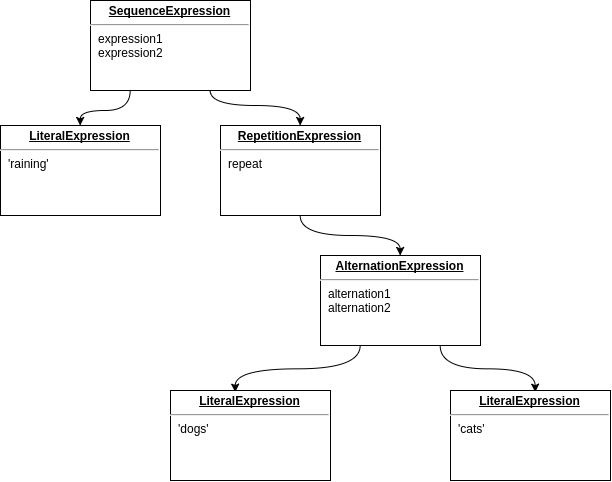
\includegraphics[width=\textwidth]{img/Interpreter-Pattern-AST-Example}
	\caption{Example in \cite{GHJV94} for the AST of regular expressions using the interpreter pattern }
	\label{fig:interpreter-pattern-ast}
\end{figure} 

Operations will be implemented in the expression class. That means that if we want to evaluate an expression, each node of the AST evaluates itself with the defined operation.

The following benefits and liabilities are described in \cite{GHJV94}:

\begin{description}
	\item[It's easy to change and extend the grammer:] Using classes to represent grammar rules allows the usage of inheritance to extend the grammar. New data types will be derived from existing ones.
	
	\item[Implementing the grammer is easy, too:] The nodes of the AST have similar functionalities, which makes the implementation easy and repetitive. This process can be automated with compiler or parser generators.
	
	\item[Complex grammars are hard to maintain:] At least one class is defined for every expression. This means that complex grammars have many different classes, which need to be maintained. Adding a new operation on these classes means one needs to change every class accordingly.
\end{description}

So as one can see the interpreter is great for grammars that are rather simple and don't change much. Extending the grammar is easy, but adding new operations is not. Object algebra uses the terms \emph{data variation} and \emph{operations}. By using these terms one can briefly summarize the interpreter as a good way to handle data variations to a certain extend (not too complex grammars), but adding new operations to expressions can easily lead to many changes as every class of each expression needs an implementation of the new operation.

\subsection{Visitor Pattern} \label{ssec:visitor}
Unlike the interpreter pattern the intent of the visitor pattern is to represent operations, which will be performed on the nodes of an AST \cite{GHJV94}.

With the visitor pattern, you define two class hierarchies. One is for the elements (or data variations) being operated on and one for the visitors that define operations on the elements \cite{GHJV94}. 

That means that if one wants to add a new operation there needs to be a new visitor class.

Data variations need a function to \emph{accept} a visitor. This accept function is no more than a callback, which calls the \emph{visit} function of the visitor, where the parameter is the data variations object. With that information the visitor knows which kind of node of the AST he is visiting and which exact function he needs to call to operate on this particular node. An example of this mechanic is shown in \autoref{fig:visitor-pattern}.

\begin{figure}[h]
	\centering
	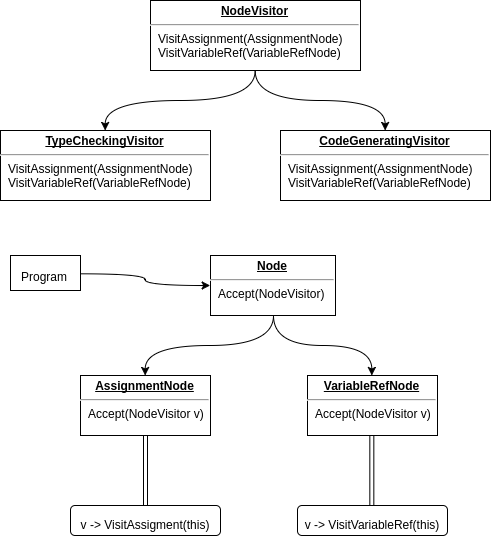
\includegraphics[width=0.8\textwidth]{img/Visitor-Pattern-Example}
	\caption{Example in \cite{GHJV94} for the visitor pattern}
	\label{fig:visitor-pattern}
\end{figure} 

In \cite{GHJV94} are the following benefits and liabilities described for the visitor pattern:

\begin{description}
	\item[Visitor makes adding new operations easy:] New operations are defined as new visitor classes. This way one doesn't need to change each class of your object structure.
	
	\item[A visitor gathers related operations and separates unrelated ones:] As a visitor represents an operation over a node of the AST, the operations are separated in different visitor classes. That means that the basic \emph{separation of concern} principle is handled by design.
	
	\item[Adding new ConcreteElement classes is hard:] On the other hand, adding a new data variation is hard, as each visitor needs to handle this new data variation. Additionally the data variation needs to \emph{accept} each visitor as well. This is not suited for structures with frequent changes of data variations and their hierarchy.
	
	\item[Visiting across class hierarchies:] Iterators can't work across object structures with different types of elements. The visitor however can because of the visit functions, which accept certain types of data variations. These data variations don't have to be related through inheritance.
	
	\item[Accumulating state:] The state of a data variation is implicitly passed as an argument to the visitor. Therefore there is no need for extra arguments or global variables in the visit function.
	
	\item[Breaking encapsulation:] The visitor pattern assumes that the interface of the data variations lets the visitors do their job. This might lead to public functions that allow access to the internal state of a data variation.
\end{description}

The \emph{double-dispatch} mechanism (accept and visit function) mentioned in \cite{GHJV94} is required if the visitor is called by the data variation. Terence Parr showed in \cite{Parr09} how one can create an independent visitor, that distinguished the different nodes of an AST on the token type, which ANTLR uses in the grammar. Switching between the types allows the visitor to traverse the AST and identify each node.

This external visitor has, according to \cite{Parr09}, some advantages as the method names can be named relevant to the task (instead of \emph{visit}) and there is no need for an interface for the visitor. The double-dispatch mechanism is also encapsulated in the visitor and not in the data variation and operation (which is here represented by the visitor). 


\subsection{Object Algebra} \label{ssec:oa}
Another solution to the \emph{expression problem} was proposed by \cite{Oliveira12} and uses \emph{object algebra}. Object algebra is based on \emph{algebraic signatures} \cite{Guttag78} and only uses \emph{constructors}, which return values of the abstract set. The abstract set in object algebras is based on \emph{data variants} and \emph{operations}. 

An example of these variants and operations is shown in \autoref{fig:oa-variants-operations} for our LTL set. So every operation is available to every data variant. Implementing object algebras is done by creating a generic interface whose parameter is the abstract type \cite{Oliveira12}. The object algebra therefore declares generic factory interfaces for the variants and factories with the variant as type for implementing the operations. This will be shown more detailed in \autoref{sec:oa-ltl} with the example set of LTL.

\begin{figure}[h]
	\centering
	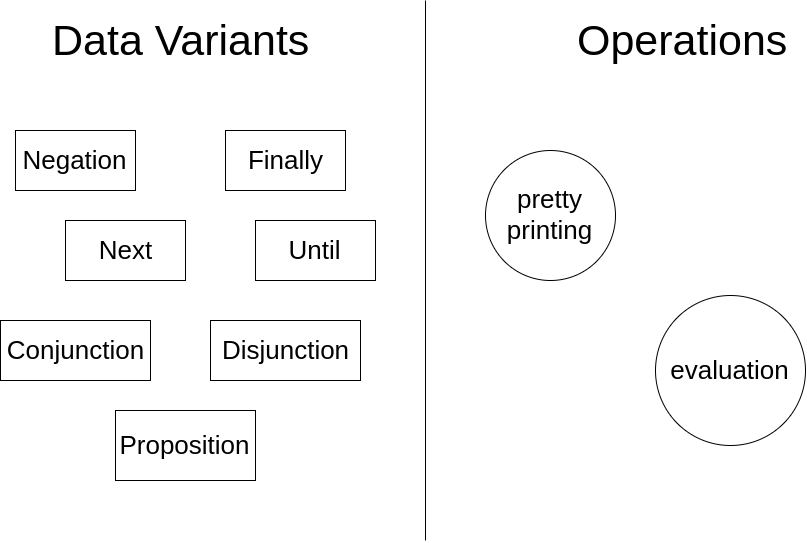
\includegraphics[width=0.65\textwidth]{img/OA-Variants-Operations}
	\caption{Example of data variants and operations used in object algebra}
	\label{fig:oa-variants-operations}
\end{figure} 

Object Algebra is similar to the \emph{visitor} pattern as both decouple \emph{variants} and \emph{operations}. The visitor pattern has visitor classes for operations and the AST nodes as variants while object algebra uses generic factory interfaces to represent expressions (variants) and factories for operations. The main difference is that the visitor pattern focuses on operations. Object algebra uses the factory style to encapsulate the operations of an abstract expression. So to add new variants one needs to extend the interface of the generic factory, which is a natural and easy object-oriented approach. To add new operations one needs to implement this generic factory interface. So the methods used are simple object-oriented methods. This also allows for the usage of \emph{polymorphism}.

To summarize it:

\begin{description}
	\item[Data type (data variant):] The data variant is a generic factory interface.
	\item[Operation:] The operation is a factory implementation.
	\item[Adding new variants: ] Adding new variants is done by extending the interface.
	\item[Adding new operations:] Adding new operations is done by implementing the interface.
\end{description}


\section{Object Algebra to the LTL Expression Problem} \label{sec:oa-ltl}
In this section we will show how one can handle the LTL expression problem using object algebra. The data variants and operations are the same as shown in \autoref{fig:oa-variants-operations}. The code is public on github\footnote{\href{https://github.com/hadesrofl/oaltl}{https://github.com/hadesrofl/oaltl}}.

\subsection{LTL Set} \label{ssec:ltl-set}
The set of LTL expressions includes \emph{conjunction, disjunction, negation, next, until, finally, atomic propositions}. To show the extensibility of object algebras \emph{finally} was added later in the development.

The operations on these expressions started with \emph{pretty printing} and were extended with the operation to \emph{evaluate} a LTL formula. The extensions of \emph{evaluate} also shows the extensibility of operations in terms of object algebra.

\subsection{Implementation} \label{ssec:implementation}
%TODO: change footnote links from develop branch to master
The implementation uses an \emph{ObjectAlgebraFactory}\footnote{\href{https://github.com/hadesrofl/oaltl/blob/develop/src/main/java/de/uzl/hsr/oaltl/ObjectAlgebraFactory.java}{Github: ObjectAlgebraFactory.java}} to force the implementation of the data variants. So this abstract interface handles the data variants. The operations got an interface e.g. \emph{PrintingObject}\footnote{\href{https://github.com/hadesrofl/oaltl/blob/develop/src/main/java/de/uzl/hsr/oaltl/PrintingObject.java}{Github: PrintingObject.java}} for the pretty printing operation. This interface defines all needed functions with its parameters in an abstract way so that the \emph{PrintingObjectFactory}\footnote{\href{https://github.com/hadesrofl/oaltl/blob/develop/src/main/java/de/uzl/hsr/oaltl/PrintingObjectFactory.java}{Github: PrintingObjectFactory.java}} needs to implement these functions of the \emph{PrintingObject} for each data variant of the \emph{ObjectAlgebraFactory}. 

%\begin{lstlisting}[caption=Implementation of the ObjectAlgebraFactory for the data variants, label=lst:object-algebra-factory]
%	package de.uzl.hsr.oaltl;
%	
%	public interface ObjectAlgebraFactory<T> {
%		public T next(T child);
%		public T fin(T child);
%		public T until(T child1, T child2);
%		public T neg(T child);
%		public T and(T child1, T child2);
%		public T or(T child1, T child2);
%		public T val(boolean val);
%		public T var(String varName);
%	}
%\end{lstlisting}

%\begin{lstlisting}[caption=PrintingObject interface for the pretty printing operation, label=lst:printing-object]
%	public interface PrintingObject {
%		public String print();
%	}
%\end{lstlisting}

%\begin{lstlisting}[caption=shorted version of the PrintingObjectFactory implementation, label=lst:printing-object-factory]
%	package de.uzl.hsr.oaltl;
%	public class PrintingObjectFactory implements 
%		ObjectAlgebraFactory<PrintingObject> {
%	
%		public PrintingObject next(PrintingObject child) {
%			return new PrintingObject() {
%				public String print() {
%					return "X(" + child.print() + ")";
%				}
%			};
%		}
%		...
%	}
%\end{lstlisting}

\begin{figure}[h]
	\centering
	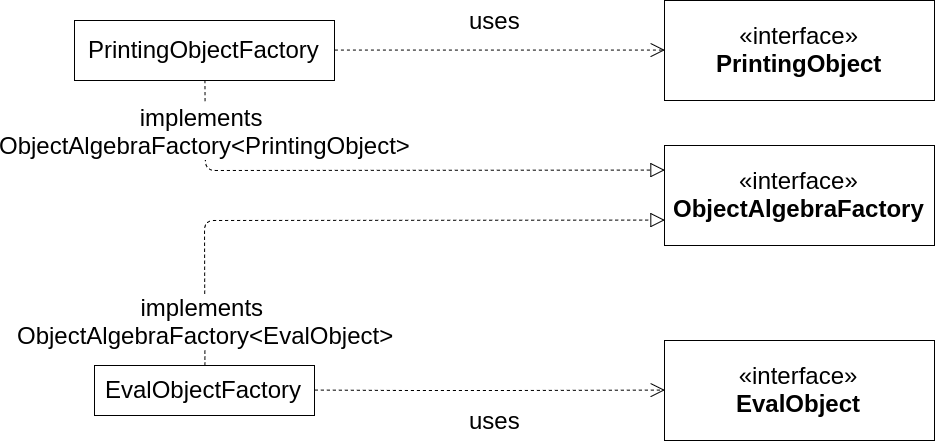
\includegraphics[width=0.8\textwidth]{img/OA-LTL-Implementation}
	\caption{Overview of the classes needed for the LTL implementation using object algebra}
	\label{fig:oa-ltl-implementation}
\end{figure} 

One can see that using this structure of object-orientation encapsulates the exact implementation of operation and data variants in a single factory for each operation. The interfaces ensure that all implementing classes are forced to implement the defined variants and also the operation. 

In our example we ended up with adding the \emph{finally} variant in the \emph{ObjectAlgebraFactory}, but instead of this way to handle the extension, one could also just extend \emph{ObjectAlgebraFactory} by something like \emph{FinallyAlgebraFactory}. So the \emph{PrintingObjectFactory} for example would implement \emph{FinallyAlgebraFactory\textless PrintingObject\textgreater} and therefore all data variants defined in ObjectAlgebraFactory as well as the new \emph{finally} addition.


\section{Conclusion} \label{sec:conclusion}
To summarize \autoref{ssec:interpreter}, the interpreter pattern is good for adding new data variants but adding new operations is difficult. Also the operations are scattered as they are implemented by each node of the AST. So the big drawback is the focus on implementing data variants and the operations being implemented in each node.

As mentioned in \autoref{ssec:visitor} the visitor pattern focuses on operations and therefore is good for adding new operations. It is also possible to read the internal state of the node the visitor is processing and generate an operation state out of this information. On the other hand it is hard to add new variants. Another point is that it generally uses the \emph{double-dispatch} mechanism, which needs the variants to implement an \emph{accept} method additionally to the already needed \emph{visit} method. Also some functions or informations of the variants need to be public so that the visitor can do his work, which breaks the encapsulation of these element information.

In \autoref{sec:oa-ltl} the general features and advantages of object algebra were shown. In terms of the expression problem it allows for a good (independent) extensibility while using the languages features to retain static type safety. The implementation in \autoref{ssec:implementation} showed how one can use object algebra and how difficult it is to add new operations and variants. Using simple object-oriented methods and polymorphism is enough to use the potential of object algebra. Adding new variants and operations is easily done via generic interfaces for data variants and factories for the operations. Maintenance in a shallow object hierarchy is easy as the generic interface and the factories are the core of this approach. Maintaining a deep hierarchy of extensions (for operations or variants) might be a bit harder, though this is a general problem of software-development as more files lead to a bigger code base to maintain. 

%
% ---- Bibliography ----
%
\begin{thebibliography}{5}
%

\bibitem{wadler98}
Wadler, P.:
The Expression Problem.
E-Mail Discussion (1998),
\url{http://homepages.inf.ed.ac.uk/wadler/papers/expression/expression.txt}

\bibitem{Odersky05}
Odersky, M., Zenger, M.:
Independently Extensible Solutions to the Expression Problem. 
In FOOL'05

\bibitem{pnueli77}
Pnueli, A.:
The temporal logic of programs.
In 18th Annual Symposium on Foundations of Computer Science, Providence, Rhode Island, USA, 31 October - 1 November 1977, pages 46-57, IEEE Computer Society, 1977

\bibitem{GHJV94}
Gamma, E., Helm R., Johnson R. and Vlissides J.:
Design Patterns: Elements of Reusable Object-Oriented Software.
Addison-Wesley Professional Computing Series, Pearson Education, 1994

\bibitem{Parr09}
Parr, T.:
Language Implementation Patterns: Create Your Own Domain-Specific and General Programming Languages.
Pragmatic Bookshelf, 2009

\bibitem{Oliveira12}
Oliveira, B., Cook, W.:
Extensibility for the Masses - Practical Extensibility with Object Algebras.
In ECOOP 2012 -- Object-Oriented Programming: 26th European Conference, Beijing, China, June 11-16, 2012, pages 2-27, Springer Berlin Heidelberg

\bibitem{Guttag78}
Guttag, J., Horning, J.:
The algebraic specification of abstract data types.
In Acta Informatica Vol. 10, pages 27-52, March 1978

\end{thebibliography}
\end{document}
